\section{Versuchsaufbau}

\subsection{Versuchsaufbau}
Die Abbildung \ref{fig:aufbau} zeigt die Apparatur, die zur Bestimmung der Molwärme von Kupfer verwendet wird. 

\begin{figure}[h!]
	\centering
	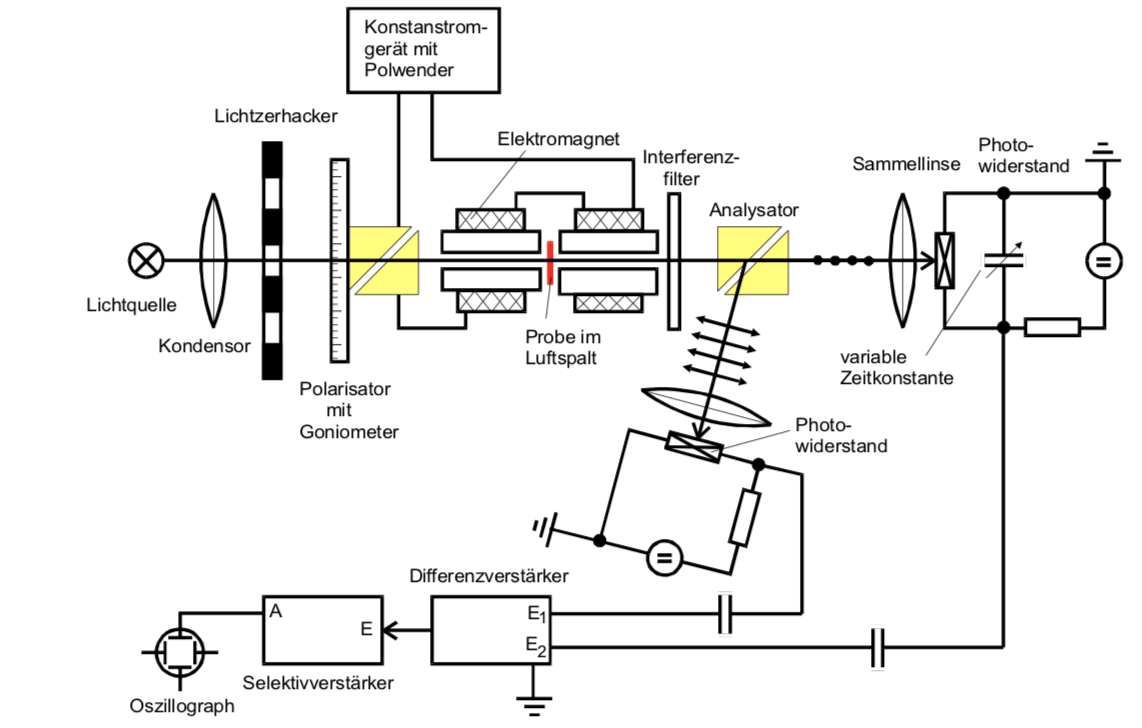
\includegraphics[width=0.7\linewidth]{../aufbau}
	\caption{Versuchsapparatur, \cite[]{anleitungV47}.}
	\label{fig:aufbau}
\end{figure}

Der Versuchsaufbau besteht aus einem Dewar-Gefäß. In dieses Gefäß wird im Laufe des Experiments flüssiges Stickstoff gefüllt. Im Inneren des Gefäßes befindet sich der Rezipient, in dem die Kupferprobe eingelagert ist. Diese Kupferprobe besitzt eine eigene Heizwicklung, welche ihrerseits von einem Kupfer-Zylinder mit Heizwicklung umgeben ist. An der Probe und dem Zylinder sind jeweils ein PT-100 Messwiderstand befestigt, der zur Bestimmung der Temperatur benötigt wird. Deren Widerstand ist eine monotone Funktion der Temperatur, diese lässt sich über die Gleichung $T=0,00134R^2+2,296R-243,02$ bestimmen. Beim Widerstandsthermometer variiert der elektrische Widerstand eines elektrischen Leiters mit der Temperatur. Weiterhin ist der Rezipient an einer Vakuumpumpe und Heliumflasche angeschlossen ist. Der Rezipient wird während des Abkühlens der Probe mit Helium befüllt. Die Erhitzung der Probe und des Zylinders erfolgen über die verbundene Stromversorgung und Heizspannung U. 

\subsection{Durchführung}
Zunächst wird der Rezipient evakuiert. Da Luft aus ca. 80 $\%$ Stickstoff besteht und die Probe mit flüssigem Stickstoff abgekühlt wird, würde sich der Stickstoff aus der Luft verflüssigen. Anschließend wird Helium bei Barometerdruck in den Rezipient gefüllt, da es eine gute thermische Leitfähigkeit aufweist, und mit Hilfe des flüssigen Stickstoffs im Dewar Gefäß wird die Probe auf 80 K abgekühlt. Helium eignet sich deshalb so gut, weil es einen niedrigeren Siedepunkt als Luft besitzt und sich bei der Abkühlung nicht verflüssigt im Gegensatz zu Luft. Nach ca. einer Stunde ist die Endtemperatur erreicht und das Rezipient wird evakuiert, um den Innendruck zu veringern, um Wärmeverluste zu vermeiden. Die Wärmeverluste können dabei Konduktion, Konvektion, Evaporation oder Strahlung sein. Anschließend wird der abgekühlten Probe elektrische Energie über die Heizwicklung zugeführt. Die Temperaturerhöhung $\Delta T$ wird über die Widerstände gemessen. Dabei soll $\Delta T$ zwischen 7$^{\circ}$ und 11$^{\circ}$ betragen. Der Kupfer-Zylinder sollte während des gesamten Versuches die gleiche Temperatur wie die Probe aufweisen, um so den Wärmeverlust aufgrund der Wärmübertragung durch einen Temperaturgradienten zu verhindern. Um dies zu ermöglichen, ist der Kupfer Zylinder an eigener Stromversorgung angeschlossen, damit elektrische Energie zugeführt werden kann. Ziel der Messung ist es die Molwärme von Kupfer für verschiedene Temperaturen zwischen 80 bis 300 Kelvin zu ermitteln. Dazu wird die Probe im Zeitabstand von fünf Minuten regelmäßig über die Stromstärke erhitzt. Währenddessen wird die Temperatur, die Messzeit, die Spannung und der Heizstrom bei konstantem Volumen notiert.  